% Options for packages loaded elsewhere
\PassOptionsToPackage{unicode}{hyperref}
\PassOptionsToPackage{hyphens}{url}
%
\documentclass[
  ignorenonframetext,
  aspectratio=169,
]{beamer}
\usepackage{pgfpages}
\setbeamertemplate{caption}[numbered]
\setbeamertemplate{caption label separator}{: }
\setbeamercolor{caption name}{fg=normal text.fg}
\beamertemplatenavigationsymbolsempty
% Prevent slide breaks in the middle of a paragraph
\widowpenalties 1 10000
\raggedbottom
\setbeamertemplate{part page}{
  \centering
  \begin{beamercolorbox}[sep=16pt,center]{part title}
    \usebeamerfont{part title}\insertpart\par
  \end{beamercolorbox}
}
\setbeamertemplate{section page}{
  \centering
  \begin{beamercolorbox}[sep=12pt,center]{part title}
    \usebeamerfont{section title}\insertsection\par
  \end{beamercolorbox}
}
\setbeamertemplate{subsection page}{
  \centering
  \begin{beamercolorbox}[sep=8pt,center]{part title}
    \usebeamerfont{subsection title}\insertsubsection\par
  \end{beamercolorbox}
}
\AtBeginPart{
  \frame{\partpage}
}
\AtBeginSection{
  \ifbibliography
  \else
    \frame{\sectionpage}
  \fi
}
\AtBeginSubsection{
  \frame{\subsectionpage}
}
\usepackage{lmodern}
\usepackage{amssymb,amsmath}
\usepackage{ifxetex,ifluatex}
\ifnum 0\ifxetex 1\fi\ifluatex 1\fi=0 % if pdftex
  \usepackage[T1]{fontenc}
  \usepackage[utf8]{inputenc}
  \usepackage{textcomp} % provide euro and other symbols
\else % if luatex or xetex
  \usepackage{unicode-math}
  \defaultfontfeatures{Scale=MatchLowercase}
  \defaultfontfeatures[\rmfamily]{Ligatures=TeX,Scale=1}
\fi
% Use upquote if available, for straight quotes in verbatim environments
\IfFileExists{upquote.sty}{\usepackage{upquote}}{}
\IfFileExists{microtype.sty}{% use microtype if available
  \usepackage[]{microtype}
  \UseMicrotypeSet[protrusion]{basicmath} % disable protrusion for tt fonts
}{}
\makeatletter
\@ifundefined{KOMAClassName}{% if non-KOMA class
  \IfFileExists{parskip.sty}{%
    \usepackage{parskip}
  }{% else
    \setlength{\parindent}{0pt}
    \setlength{\parskip}{6pt plus 2pt minus 1pt}}
}{% if KOMA class
  \KOMAoptions{parskip=half}}
\makeatother
\usepackage{xcolor}
\IfFileExists{xurl.sty}{\usepackage{xurl}}{} % add URL line breaks if available
\IfFileExists{bookmark.sty}{\usepackage{bookmark}}{\usepackage{hyperref}}
\hypersetup{
  pdftitle={Pulling and processing the data},
  hidelinks,
  pdfcreator={LaTeX via pandoc}}
\urlstyle{same} % disable monospaced font for URLs
\newif\ifbibliography
\usepackage{color}
\usepackage{fancyvrb}
\newcommand{\VerbBar}{|}
\newcommand{\VERB}{\Verb[commandchars=\\\{\}]}
\DefineVerbatimEnvironment{Highlighting}{Verbatim}{commandchars=\\\{\}}
% Add ',fontsize=\small' for more characters per line
\usepackage{framed}
\definecolor{shadecolor}{RGB}{248,248,248}
\newenvironment{Shaded}{\begin{snugshade}}{\end{snugshade}}
\newcommand{\AlertTok}[1]{\textcolor[rgb]{0.94,0.16,0.16}{#1}}
\newcommand{\AnnotationTok}[1]{\textcolor[rgb]{0.56,0.35,0.01}{\textbf{\textit{#1}}}}
\newcommand{\AttributeTok}[1]{\textcolor[rgb]{0.77,0.63,0.00}{#1}}
\newcommand{\BaseNTok}[1]{\textcolor[rgb]{0.00,0.00,0.81}{#1}}
\newcommand{\BuiltInTok}[1]{#1}
\newcommand{\CharTok}[1]{\textcolor[rgb]{0.31,0.60,0.02}{#1}}
\newcommand{\CommentTok}[1]{\textcolor[rgb]{0.56,0.35,0.01}{\textit{#1}}}
\newcommand{\CommentVarTok}[1]{\textcolor[rgb]{0.56,0.35,0.01}{\textbf{\textit{#1}}}}
\newcommand{\ConstantTok}[1]{\textcolor[rgb]{0.00,0.00,0.00}{#1}}
\newcommand{\ControlFlowTok}[1]{\textcolor[rgb]{0.13,0.29,0.53}{\textbf{#1}}}
\newcommand{\DataTypeTok}[1]{\textcolor[rgb]{0.13,0.29,0.53}{#1}}
\newcommand{\DecValTok}[1]{\textcolor[rgb]{0.00,0.00,0.81}{#1}}
\newcommand{\DocumentationTok}[1]{\textcolor[rgb]{0.56,0.35,0.01}{\textbf{\textit{#1}}}}
\newcommand{\ErrorTok}[1]{\textcolor[rgb]{0.64,0.00,0.00}{\textbf{#1}}}
\newcommand{\ExtensionTok}[1]{#1}
\newcommand{\FloatTok}[1]{\textcolor[rgb]{0.00,0.00,0.81}{#1}}
\newcommand{\FunctionTok}[1]{\textcolor[rgb]{0.00,0.00,0.00}{#1}}
\newcommand{\ImportTok}[1]{#1}
\newcommand{\InformationTok}[1]{\textcolor[rgb]{0.56,0.35,0.01}{\textbf{\textit{#1}}}}
\newcommand{\KeywordTok}[1]{\textcolor[rgb]{0.13,0.29,0.53}{\textbf{#1}}}
\newcommand{\NormalTok}[1]{#1}
\newcommand{\OperatorTok}[1]{\textcolor[rgb]{0.81,0.36,0.00}{\textbf{#1}}}
\newcommand{\OtherTok}[1]{\textcolor[rgb]{0.56,0.35,0.01}{#1}}
\newcommand{\PreprocessorTok}[1]{\textcolor[rgb]{0.56,0.35,0.01}{\textit{#1}}}
\newcommand{\RegionMarkerTok}[1]{#1}
\newcommand{\SpecialCharTok}[1]{\textcolor[rgb]{0.00,0.00,0.00}{#1}}
\newcommand{\SpecialStringTok}[1]{\textcolor[rgb]{0.31,0.60,0.02}{#1}}
\newcommand{\StringTok}[1]{\textcolor[rgb]{0.31,0.60,0.02}{#1}}
\newcommand{\VariableTok}[1]{\textcolor[rgb]{0.00,0.00,0.00}{#1}}
\newcommand{\VerbatimStringTok}[1]{\textcolor[rgb]{0.31,0.60,0.02}{#1}}
\newcommand{\WarningTok}[1]{\textcolor[rgb]{0.56,0.35,0.01}{\textbf{\textit{#1}}}}
\setlength{\emergencystretch}{3em} % prevent overfull lines
\providecommand{\tightlist}{%
  \setlength{\itemsep}{0pt}\setlength{\parskip}{0pt}}
\setcounter{secnumdepth}{-\maxdimen} % remove section numbering
%---------------------------------------------------------------------------
% BeamerHead.sty
%---------------------------------------------------------------------------
\usepackage{ifxetex,ifluatex}

%---------------------------------------------------------------------------
% General
%---------------------------------------------------------------------------
\usepackage{setspace}
\setstretch{1.25}

%\usepackage[T1]{fontenc} % Use 8-bit encoding that has 256 glyphs
% \usepackage[utf8]{inputenc}
% \usepackage{lmodern}

%\usepackage{fourier} % Use the Adobe Utopia font for the document - comment this line to return to the LaTeX default

% \setbeamerfont{item}{size*={7.5}{8}}
% \setbeamerfont{item projected}{size*={7.5}{8}}
% \setbeamerfont{itemize item}{size*={7.5}{8}}
% \setbeamerfont{itemize subitem}{size*={7.5}{8}}
% \setbeamerfont{itemize subsubitem}{size*={7.5}{8}}
% \setbeamerfont{itemize/enumerate body}{size*={7.5}{8}}
% \setbeamerfont{itemize/enumerate subbody}{size*={7.5}{8}}
% \setbeamerfont{itemize/enumerate subsubbody}{size*={7.5}{8}}
% \setbeamerfont{caption}{size*={7.5}{8}}
% \setbeamerfont{caption name}{size*={7.5}{8}}
% \setbeamerfont{frametitle}{size*={9}{9.5}}
% \setbeamerfont{normal text}{size*={7.5}{8}}
% Smaller itemize bullets
\setbeamertemplate{itemize items}{
	\raisebox{0.15\height}{$\vcenter{\hbox{\scalebox{0.5}{
	\usebeamercolor[fg]{structure} $\blacktriangleright$}}}$}}

%\usepackage{sectsty} % Allows customizing section commands
%\allsectionsfont{\centering \normalfont\scshape} % Make all sections centered, the default font and small caps
%\numberwithin{equation}{section} % Number equations within sections
%\numberwithin{figure}{section} % Number figures within sections
%\numberwithin{table}{section} % Number tables within sections

\usepackage{multicol}
\setlength{\columnsep}{20pt}
\newlength\Colsep

%---------------------------------------------------------------------------
% Header/footer
%---------------------------------------------------------------------------
\setbeamertemplate{navigation symbols}{}
\setbeamertemplate{footline}[page number]

%---------------------------------------------------------------------------
% Citations
%---------------------------------------------------------------------------
% \usepackage[backend=bibtex]{biblatex}

%---------------------------------------------------------------------------
% Tables, figures, images
%---------------------------------------------------------------------------
\usepackage{wrapfig}
\usepackage{longtable}
\setlength{\LTcapwidth}{\textwidth}
\usepackage{xtab, booktabs}
\usepackage{multirow}

\usepackage{tikz}% Probability trees and flow charts and the like
\usetikzlibrary{%
trees,
arrows,
shapes,
%decoration,
automata,
backgrounds,
petri}

% Witin cell wrapping
% https://tex.stackexchange.com/questions/2441/how-to-add-a-forced-line-break-inside-a-table-cell
\usepackage{makecell}
\renewcommand\theadalign{bc}
\renewcommand\theadfont{\bfseries}
\renewcommand\theadgape{\Gape[4pt]}
\renewcommand\cellgape{\Gape[4pt]}
% Usage
% \thead{Two line \\ head}
% \makecell{Some really \\ longer text}

% \usepackage{graphicx,grffile}
% For tables and figures in parts %%%%
\usepackage{caption}
\DeclareCaptionLabelFormat{cont}{#1~#2\alph{ContinuedFloat}}
% \usepackage{subcaption}
% \captionsetup{font=scriptsize,labelfont=scriptsize}
%\graphicspath{ {file.path.here} }

% \usepackage{subfloat}

% Set column widths in tabular environment!
\usepackage{array}
\newcommand{\PreserveBackslash}[1]{\let\temp=\\#1\let\\=\temp}
\newcolumntype{C}[1]{>{\PreserveBackslash\centering}p{#1}}
\newcolumntype{R}[1]{>{\PreserveBackslash\raggedleft}p{#1}}
\newcolumntype{L}[1]{>{\PreserveBackslash\raggedright}p{#1}}

% Fancy fit image command with optional caption
\usepackage{adjustbox} % Shrink stuff
% \usepackage{showframe} % Useful for debugging

%---------------------------------------------------------------------------
% Typographical addendum
%---------------------------------------------------------------------------
\input{\string~/HeadRs/common_supplement.tex}

\title{Pulling and processing the data}
\subtitle{GM-UAW Cohort Study}
\author{}
\date{\vspace{-2.5em}\today}

\begin{document}
\frame{\titlepage}

\begin{frame}[fragile]{Overview}
\protect\hypertarget{overview}{}

\begin{itemize}
\tightlist
\item
  Pulling and preliminary cleaning
\item
  Building analytic dataset

  \begin{itemize}
  \tightlist
  \item
    Demographic data in person-time format
  \item
    Map ICD codes to causes of death/cancer types
  \item
    Merge exposure data and job history data
  \end{itemize}
\item
  Intermediate objects are saved in
  \href{https://berkeley.app.box.com/folder/113431246688}{Box folder
  113431246688}
\item
  \texttt{R} code for doing all of this on
  \href{https://github.com/tao-feng/gm-wrangling.git}{Github}
\end{itemize}

\end{frame}

\begin{frame}{Pulling and preliminary cleaning}
\protect\hypertarget{pulling-and-preliminary-cleaning}{}

\begin{minipage}{\linewidth}
    \centering
    \begin{adjustbox}{scale = 0.7}
    
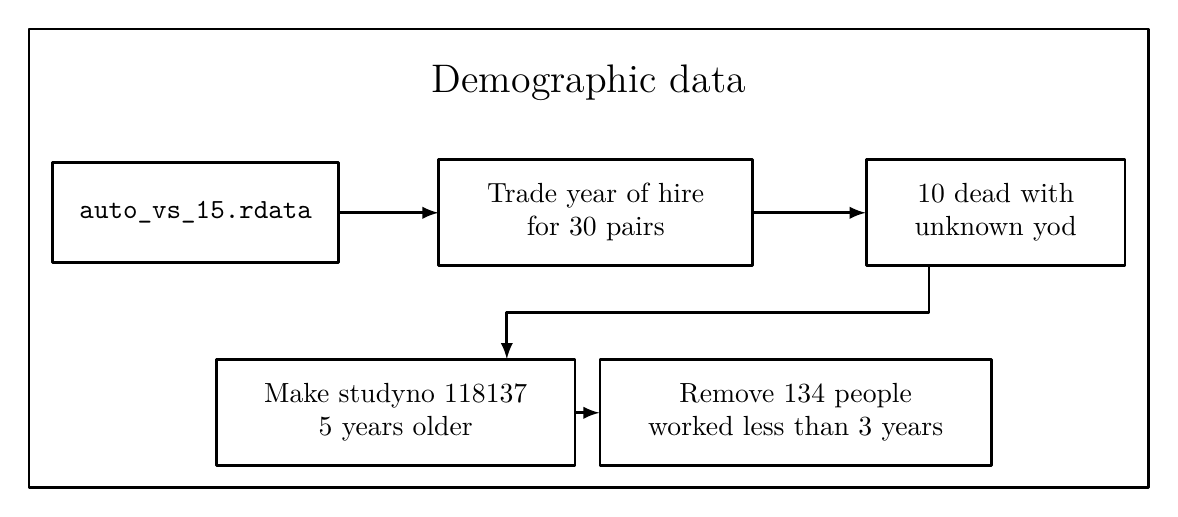
\begin{tikzpicture}[>=latex,line join=bevel,]
  \pgfsetlinewidth{1bp}
%%
\begin{scope}
  \pgfsetstrokecolor{black}
  \definecolor{strokecol}{rgb}{0.0,0.0,0.0}
  \pgfsetstrokecolor{strokecol}
  \draw (-0.26bp,0.14bp) -- (-0.26bp,165.14bp) -- (402.74bp,165.14bp) -- (402.74bp,0.14bp) -- cycle;
  \draw (201.24bp,145.64bp) node {\Large Demographic data};
\end{scope}
  \pgfsetcolor{black}
  % Edge: unknownDeath -> unusuYoung
  \draw [->] (323.74bp,79.801bp) .. controls (323.74bp,71.208bp) and (323.74bp,63.0bp)  .. (323.74bp,63.0bp) .. controls (323.74bp,63.0bp) and (171.74bp,63.0bp)  .. (171.74bp,63.0bp) .. controls (171.74bp,63.0bp) and (171.74bp,56.33bp)  .. (171.74bp,46.33bp);
  % Edge: unusuYoung -> removeImmortals
  \draw [->] (196.58bp,27.0bp) .. controls (196.58bp,27.0bp) and (197.43bp,27.0bp)  .. (205.11bp,27.0bp);
  % Edge: dem -> admin
  \draw [->] (111.32bp,99.0bp) .. controls (111.32bp,99.0bp) and (137.15bp,99.0bp)  .. (147.15bp,99.0bp);
  % Edge: admin -> unknownDeath
  \draw [->] (260.65bp,99.0bp) .. controls (260.65bp,99.0bp) and (290.97bp,99.0bp)  .. (300.97bp,99.0bp);
  % Node: admin
\begin{scope}
  \definecolor{strokecol}{rgb}{0.0,0.0,0.0}
  \pgfsetstrokecolor{strokecol}
  \draw (260.24bp,118.14bp) -- (147.24bp,118.14bp) -- (147.24bp,80.14bp) -- (260.24bp,80.14bp) -- cycle;
  \draw (203.74bp,99.141bp) node {\begin{tabular}{c}
							Trade year of hire \\							for 30 pairs \end{tabular}};
\end{scope}
  % Node: unusuYoung
\begin{scope}
  \definecolor{strokecol}{rgb}{0.0,0.0,0.0}
  \pgfsetstrokecolor{strokecol}
  \draw (196.24bp,46.14bp) -- (67.24bp,46.14bp) -- (67.24bp,8.14bp) -- (196.24bp,8.14bp) -- cycle;
  \draw (131.74bp,27.141bp) node {\begin{tabular}{c}
							Make studyno 118137 \\							5 years older \end{tabular}};
\end{scope}
  % Node: unknownDeath
\begin{scope}
  \definecolor{strokecol}{rgb}{0.0,0.0,0.0}
  \pgfsetstrokecolor{strokecol}
  \draw (394.24bp,118.14bp) -- (301.24bp,118.14bp) -- (301.24bp,80.14bp) -- (394.24bp,80.14bp) -- cycle;
  \draw (347.74bp,99.141bp) node {\begin{tabular}{c}
							10 dead with \\							unknown yod \end{tabular}};
\end{scope}
  % Node: dem
\begin{scope}
  \definecolor{strokecol}{rgb}{0.0,0.0,0.0}
  \pgfsetstrokecolor{strokecol}
  \draw (111.24bp,117.14bp) -- (8.24bp,117.14bp) -- (8.24bp,81.14bp) -- (111.24bp,81.14bp) -- cycle;
  \draw (59.738bp,99.141bp) node {\texttt{auto\_vs\_15.rdata}};
\end{scope}
  % Node: removeImmortals
\begin{scope}
  \definecolor{strokecol}{rgb}{0.0,0.0,0.0}
  \pgfsetstrokecolor{strokecol}
  \draw (346.24bp,46.14bp) -- (205.24bp,46.14bp) -- (205.24bp,8.14bp) -- (346.24bp,8.14bp) -- cycle;
  \draw (275.74bp,27.141bp) node {\begin{tabular}{c}
							Remove 134 people \\							worked less than 3 years \end{tabular}};
\end{scope}
%
\end{tikzpicture}


    \end{adjustbox}
\end{minipage}\vspace{1em}
\begin{minipage}{\linewidth}
    \centering
    \begin{adjustbox}{scale = 0.7}
    
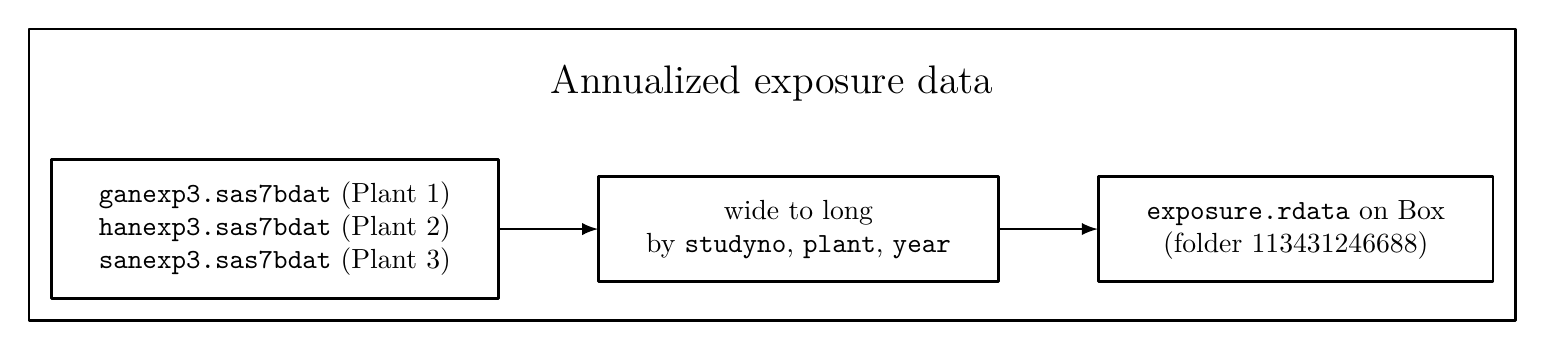
\begin{tikzpicture}[>=latex,line join=bevel,]
  \pgfsetlinewidth{1bp}
%%
\begin{scope}
  \pgfsetstrokecolor{black}
  \definecolor{strokecol}{rgb}{0.0,0.0,0.0}
  \pgfsetstrokecolor{strokecol}
  \draw (8.0bp,8.0bp) -- (8.0bp,113.0bp) -- (543.0bp,113.0bp) -- (543.0bp,8.0bp) -- cycle;
  \draw (275.5bp,93.5bp) node {\Large Annualized exposure data};
\end{scope}
  \pgfsetcolor{black}
  % Edge: exposure -> long
  \draw [->] (177.13bp,41.0bp) .. controls (185.58bp,41.0bp) and (194.18bp,41.0bp)  .. (212.89bp,41.0bp);
  % Edge: long -> final
  \draw [->] (357.23bp,41.0bp) .. controls (365.56bp,41.0bp) and (374.1bp,41.0bp)  .. (392.78bp,41.0bp);
  % Node: final
\begin{scope}
  \definecolor{strokecol}{rgb}{0.0,0.0,0.0}
  \pgfsetstrokecolor{strokecol}
  \draw (535.0bp,60.0bp) -- (393.0bp,60.0bp) -- (393.0bp,22.0bp) -- (535.0bp,22.0bp) -- cycle;
  \draw (464.0bp,41.0bp) node {\begin{tabular}{c} 
						\texttt{exposure.rdata} on Box \\						({folder 113431246688})
						\end{tabular}};
\end{scope}
  % Node: long
\begin{scope}
  \definecolor{strokecol}{rgb}{0.0,0.0,0.0}
  \pgfsetstrokecolor{strokecol}
  \draw (357.0bp,60.0bp) -- (213.0bp,60.0bp) -- (213.0bp,22.0bp) -- (357.0bp,22.0bp) -- cycle;
  \draw (285.0bp,41.0bp) node {\begin{tabular}{c} 
						wide to long \\						by \texttt{studyno}, \texttt{plant}, \texttt{year}
						\end{tabular}};
\end{scope}
  % Node: exposure
\begin{scope}
  \definecolor{strokecol}{rgb}{0.0,0.0,0.0}
  \pgfsetstrokecolor{strokecol}
  \draw (177.0bp,66.0bp) -- (16.0bp,66.0bp) -- (16.0bp,16.0bp) -- (177.0bp,16.0bp) -- cycle;
  \draw (96.5bp,41.0bp) node {\begin{tabular}{c} 
						\texttt{ganexp3.sas7bdat} (Plant 1) \\						\texttt{hanexp3.sas7bdat} (Plant 2) \\						\texttt{sanexp3.sas7bdat} (Plant 3) \\						\end{tabular}};
\end{scope}
%
\end{tikzpicture}


    \end{adjustbox}
\end{minipage}

\end{frame}

\begin{frame}{}
\protect\hypertarget{section}{}

\begin{center}
    \begin{adjustbox}{scale = 0.7}
    
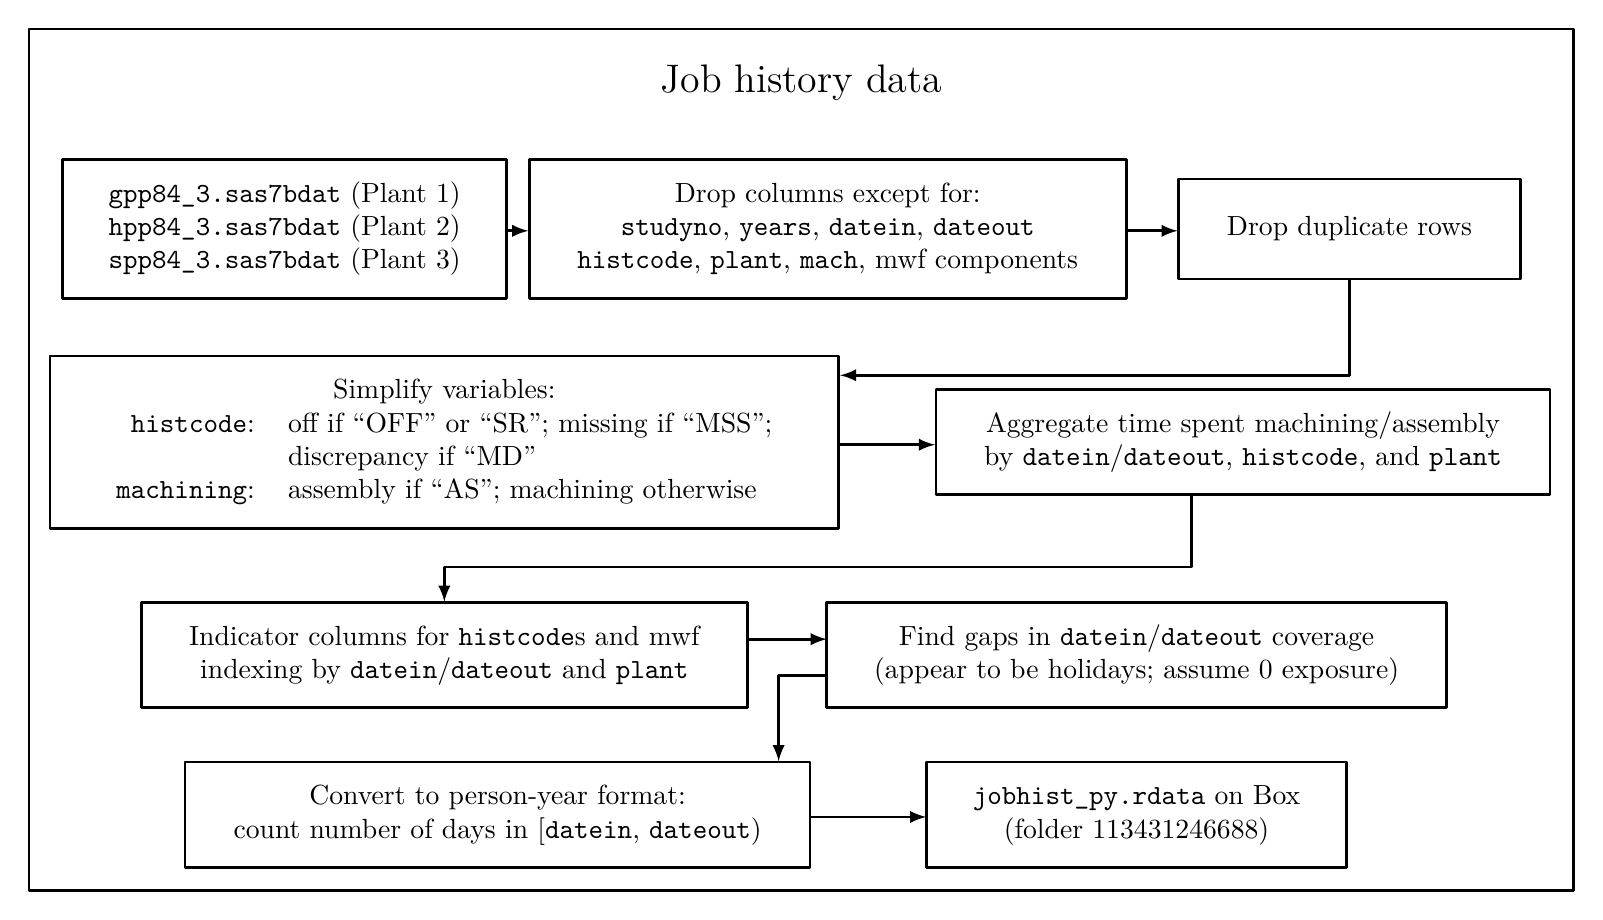
\begin{tikzpicture}[>=latex,line join=bevel,]
  \pgfsetlinewidth{1bp}
%%
\begin{scope}
  \pgfsetstrokecolor{black}
  \definecolor{strokecol}{rgb}{0.0,0.0,0.0}
  \pgfsetstrokecolor{strokecol}
  \draw (0.24bp,-0.36bp) -- (0.24bp,309.64bp) -- (556.24bp,309.64bp) -- (556.24bp,-0.36bp) -- cycle;
  \draw (278.24bp,290.14bp) node {\Large Job history data};
\end{scope}
  \pgfsetcolor{black}
  % Edge: filter -> drop
  \draw [->] (395.4bp,237.0bp) .. controls (395.4bp,237.0bp) and (403.73bp,237.0bp)  .. (413.73bp,237.0bp);
  % Edge: drop -> simplify
  \draw [->] (475.61bp,219.52bp) .. controls (475.61bp,204.3bp) and (475.61bp,185.0bp)  .. (475.61bp,185.0bp) .. controls (475.61bp,185.0bp) and (302.2bp,185.0bp)  .. (292.2bp,185.0bp);
  % Edge: machining -> histcode
  \draw [->] (418.6bp,141.9bp) .. controls (418.6bp,129.64bp) and (418.6bp,116.0bp)  .. (418.6bp,116.0bp) .. controls (418.6bp,116.0bp) and (149.74bp,116.0bp)  .. (149.74bp,116.0bp) .. controls (149.74bp,116.0bp) and (149.74bp,113.47bp)  .. (149.74bp,103.47bp);
  % Edge: job -> filter
  \draw [->] (172.33bp,237.0bp) .. controls (172.33bp,237.0bp) and (173.09bp,237.0bp)  .. (179.96bp,237.0bp);
  % Edge: simplify -> machining
  \draw [->] (291.82bp,160.0bp) .. controls (291.82bp,160.0bp) and (316.37bp,160.0bp)  .. (326.37bp,160.0bp);
  % Edge: histcode -> cont
  \draw [->] (259.04bp,90.0bp) .. controls (259.04bp,90.0bp) and (277.42bp,90.0bp)  .. (287.42bp,90.0bp);
  % Edge: cont -> clean
  \draw [->] (287.19bp,77.0bp) .. controls (276.81bp,77.0bp) and (270.08bp,77.0bp)  .. (270.08bp,77.0bp) .. controls (270.08bp,77.0bp) and (270.08bp,56.057bp)  .. (270.08bp,46.057bp);
  % Edge: clean -> final
  \draw [->] (281.57bp,26.0bp) .. controls (281.57bp,26.0bp) and (313.2bp,26.0bp)  .. (323.2bp,26.0bp);
  % Node: cont
\begin{scope}
  \definecolor{strokecol}{rgb}{0.0,0.0,0.0}
  \pgfsetstrokecolor{strokecol}
  \draw (510.44bp,103.29bp) -- (287.44bp,103.29bp) -- (287.44bp,65.29bp) -- (510.44bp,65.29bp) -- cycle;
  \draw (398.94bp,84.292bp) node {\begin{tabular}{c} 
						Find gaps in \texttt{datein}/\texttt{dateout} coverage \\						(appear to be holidays; assume 0 exposure)
						\end{tabular}};
\end{scope}
  % Node: drop
\begin{scope}
  \definecolor{strokecol}{rgb}{0.0,0.0,0.0}
  \pgfsetstrokecolor{strokecol}
  \draw (537.11bp,255.64bp) -- (414.11bp,255.64bp) -- (414.11bp,219.64bp) -- (537.11bp,219.64bp) -- cycle;
  \draw (475.61bp,237.64bp) node {\begin{tabular}{c} 
						Drop duplicate rows
						\end{tabular}};
\end{scope}
  % Node: filter
\begin{scope}
  \definecolor{strokecol}{rgb}{0.0,0.0,0.0}
  \pgfsetstrokecolor{strokecol}
  \draw (395.26bp,262.64bp) -- (180.26bp,262.64bp) -- (180.26bp,212.64bp) -- (395.26bp,212.64bp) -- cycle;
  \draw (287.76bp,237.64bp) node {\begin{tabular}{c} 
						Drop columns except for: \\						\texttt{studyno}, \texttt{years}, \texttt{datein}, \texttt{dateout} \\						\texttt{histcode}, \texttt{plant}, \texttt{mach}, mwf components \\						\end{tabular}};
\end{scope}
  % Node: simplify
\begin{scope}
  \definecolor{strokecol}{rgb}{0.0,0.0,0.0}
  \pgfsetstrokecolor{strokecol}
  \draw (291.74bp,191.97bp) -- (7.74bp,191.97bp) -- (7.74bp,129.97bp) -- (291.74bp,129.97bp) -- cycle;
  \draw (149.74bp,160.97bp) node {\begin{tabular}{c} 
						Simplify variables: \\								\begin{tabular}{rl}
								\texttt{histcode}: & off if ``OFF'' or ``SR'';
								missing if ``MSS''; \\								& discrepancy if ``MD'' \\								\texttt{machining}: & assembly if ``AS''; machining otherwise
								\end{tabular}
						\end{tabular}};
\end{scope}
  % Node: job
\begin{scope}
  \definecolor{strokecol}{rgb}{0.0,0.0,0.0}
  \pgfsetstrokecolor{strokecol}
  \draw (172.24bp,262.64bp) -- (12.24bp,262.64bp) -- (12.24bp,212.64bp) -- (172.24bp,212.64bp) -- cycle;
  \draw (92.238bp,237.64bp) node {\begin{tabular}{c} 
						\texttt{gpp84\_3.sas7bdat} (Plant 1) \\						\texttt{hpp84\_3.sas7bdat} (Plant 2) \\						\texttt{spp84\_3.sas7bdat} (Plant 3) \\						\end{tabular}};
\end{scope}
  % Node: machining
\begin{scope}
  \definecolor{strokecol}{rgb}{0.0,0.0,0.0}
  \pgfsetstrokecolor{strokecol}
  \draw (547.77bp,179.97bp) -- (326.77bp,179.97bp) -- (326.77bp,141.97bp) -- (547.77bp,141.97bp) -- cycle;
  \draw (437.27bp,160.97bp) node {\begin{tabular}{c} 
						Aggregate time spent machining/assembly \\						by \texttt{datein}/\texttt{dateout}, \texttt{histcode}, and \texttt{plant}
						\end{tabular}};
\end{scope}
  % Node: clean
\begin{scope}
  \definecolor{strokecol}{rgb}{0.0,0.0,0.0}
  \pgfsetstrokecolor{strokecol}
  \draw (281.41bp,45.79bp) -- (56.41bp,45.79bp) -- (56.41bp,7.79bp) -- (281.41bp,7.79bp) -- cycle;
  \draw (168.91bp,26.786bp) node {\begin{tabular}{c} 
						Convert to person-year format: \\						count number of days in [\texttt{datein}, \texttt{dateout})
						\end{tabular}};
\end{scope}
  % Node: histcode
\begin{scope}
  \definecolor{strokecol}{rgb}{0.0,0.0,0.0}
  \pgfsetstrokecolor{strokecol}
  \draw (258.74bp,103.29bp) -- (40.74bp,103.29bp) -- (40.74bp,65.29bp) -- (258.74bp,65.29bp) -- cycle;
  \draw (149.74bp,84.292bp) node {\begin{tabular}{c} 
						Indicator columns for \texttt{histcode}s and mwf\\						indexing by \texttt{datein}/\texttt{dateout} and \texttt{plant}
						\end{tabular}};
\end{scope}
  % Node: final
\begin{scope}
  \definecolor{strokecol}{rgb}{0.0,0.0,0.0}
  \pgfsetstrokecolor{strokecol}
  \draw (474.44bp,45.79bp) -- (323.44bp,45.79bp) -- (323.44bp,7.79bp) -- (474.44bp,7.79bp) -- cycle;
  \draw (398.94bp,26.786bp) node {\begin{tabular}{c} 
						\texttt{jobhist\_py.rdata} on Box \\						({folder 113431246688})
						\end{tabular}};
\end{scope}
%
\end{tikzpicture}


    \end{adjustbox}
\end{center}

\end{frame}

\begin{frame}[fragile]{Person-year dataset}
\protect\hypertarget{person-year-dataset}{}

\begin{itemize}
\tightlist
\item
  Start with the cleaned demographic data \texttt{cohort}
\item
  Duplicate each row so that each year from hire to death/end of FU is
  represented
\item
  Index appropriately by calendar year and age
\end{itemize}

\end{frame}

\begin{frame}[fragile]{Outcome labels}
\protect\hypertarget{outcome-labels}{}

\begin{itemize}
\tightlist
\item
  Cause of death labels coded up using ICD mappings given by the
  NIOSH-92 death categories document (linked
  \href{https://www.cdc.gov/niosh/ltas/pdf/Rate-Info-Table-3.pdf}{here})
\item
  Cancer incidence from MCR coded up by Liza (thank you!)
\item
  Cancer incidence from SEER coded up using the Site Recode ICD-O-3/WHO
  2008 Definitions (linked
  \href{https://seer.cancer.gov/siterecode/icdo3_dwhoheme/index.html}{here}),
  taking into account both the ICD-O-3 Site code \emph{and} the ICD-O-3
  Histology code

  \begin{itemize}
  \tightlist
  \item
    Cleaned up SEER incidence data frames on Box (see
    \texttt{SEER\ incidence.csv} in (folder
    113431246688){[}\url{https://berkeley.app.box.com/folder/113431246688}{]})
  \end{itemize}
\end{itemize}

\end{frame}

\begin{frame}[fragile]{Merging exposure and job history data}
\protect\hypertarget{merging-exposure-and-job-history-data}{}

\begin{itemize}
\tightlist
\item
  Recall that exposure data was indexed by \texttt{studyno},
  \texttt{year}, \emph{and} \texttt{plant}

  \begin{itemize}
  \tightlist
  \item
    Before merging, exposure was summed across plants i.e.~indexed by
    \texttt{studyno} and \texttt{year} only
  \end{itemize}
\item
  \texttt{plant} was taken to be plant with the most days in
  \texttt{jobhist\_py.rdata}, for that \texttt{year}
\end{itemize}

\end{frame}

\begin{frame}{Code: it's all on github}
\protect\hypertarget{code-its-all-on-github}{}

\begin{center}
\begin{adjustbox}{max width = 0.75\linewidth}
\href{https://github.com/tao-feng/gm-wrangling.git}{\includegraphics{resources/repo.png}}
\end{adjustbox}
\end{center}

\end{frame}

\begin{frame}[fragile]{Getting the code}
\protect\hypertarget{getting-the-code}{}

\begin{Shaded}
\begin{Highlighting}[]
\CommentTok{#!/bin/sh }

\BuiltInTok{cd} \StringTok{"~"} \CommentTok{# Must must clone into your home directory}
\FunctionTok{git}\NormalTok{ clone https://github.com/tao-feng/HeadRs.git }\CommentTok{# Dependencies}

\BuiltInTok{cd} \StringTok{"directory/of your/choice"}
\FunctionTok{git}\NormalTok{ clone https://github.com/tao-feng/gm-wrangling.git}
\end{Highlighting}
\end{Shaded}

Or Download ZIP -- after unzipping, please change the directory names to
``HeadRs'' and ``gm-wrangling''

The home directory \texttt{R} sees can be found by running
\texttt{path.expand("\textasciitilde{}")}

\end{frame}

\begin{frame}[fragile]{Getting the data and helper functions}
\protect\hypertarget{getting-the-data-and-helper-functions}{}

\begin{Shaded}
\begin{Highlighting}[]
\CommentTok{# Check that necessary packages are installed}
\KeywordTok{lapply}\NormalTok{(}\KeywordTok{c}\NormalTok{(}\StringTok{"tidyverse"}\NormalTok{, }\StringTok{"xtable"}\NormalTok{, }\StringTok{"pander"}\NormalTok{, }\StringTok{"tikzDevice"}\NormalTok{, }\StringTok{"knitr"}\NormalTok{,}
    \StringTok{"data.table"}\NormalTok{, }\StringTok{"zoo"}\NormalTok{, }\StringTok{"boxr"}\NormalTok{, }\StringTok{"lubridate"}\NormalTok{, }\StringTok{"sas7bdat"}\NormalTok{, }\StringTok{"Hmisc"}\NormalTok{),}
    \ControlFlowTok{function}\NormalTok{(package) \{}\ControlFlowTok{if}\NormalTok{ (}\OperatorTok{!}\NormalTok{package }\OperatorTok\StringTok{ }\KeywordTok{installed.packages}\NormalTok{()) \{}
        \KeywordTok{install.packages}\NormalTok{(package)\}\})}

\CommentTok{# Get data and helper functions}
\KeywordTok{source}\NormalTok{(}\StringTok{"directory/of your/choice/gm-wrangling/wrangling/00-hello.R"}\NormalTok{)}
\end{Highlighting}
\end{Shaded}

Note: Setting up \texttt{boxr} is a bit of a pain\ldots{}

\end{frame}

\begin{frame}[fragile]{What you get from running \texttt{00-hello.R}}
\protect\hypertarget{what-you-get-from-running-00-hello.r}{}

\begin{center}\begin{adjustbox}{max width = 0.85\linewidth}\ttfamily
\begin{tabular}{llll}
  \toprule
additional\_outcomes() & get.cohort\_py() & jobhist & mytheme.web \\ 
  cohort & get.exposure() & jobhist\_py & og.dir \\ 
  date.to.gm() & get.jobhist() & jobhist\_py.cast & self\_injury.function() \\ 
  death\_type() & get.ltab\_obs() & latex() & spec\_icd\_codes() \\ 
  drive\_D & gm.to.date() & ltab\_age() & tikzLualatexPackages.option \\ 
  dta & hook\_output() & ltab\_calendar() & to\_drive\_D() \\ 
  exposure & icd\_codes.function() & lualatex()  \\ 
  get.cohort\_analytic() & is.auto\_vs\_15 & mytheme  \\ 
   \bottomrule
\end{tabular}
\end{adjustbox}\end{center}

Notes

\begin{itemize}
\tightlist
\item
  \texttt{cohort} is the cleaned demographic data

  \begin{itemize}
  \tightlist
  \item
    Please check variable names and types
  \item
    Most variables correspond to those in \texttt{auto\_vs\_15}
  \end{itemize}
\item
  \texttt{exposure} is the pulled/merged exposure data
\item
  \texttt{jobhist\_py} is the cleaned person-year job history data
\end{itemize}

\end{frame}

\begin{frame}{Making the analytic data object}
\protect\hypertarget{making-the-analytic-data-object}{}

\end{frame}

\end{document}
